We already established the existence of lead--lag structures between different questions and industry codes. A central goal is therefore to identify industries that allow us to predict the main index reliably. To enhance stability, we focus not on single industries but rather on subsets of industry codes.

The central idea is to identify subsets of industries that allow reliable prediction of the main index. To this end, we construct prediction sets based on lead--lag profiles. Specifically, we distinguish between a \emph{Prediction Set}, which covers leads of one to six months, and an \emph{Early Prediction Set}, which focuses on leads of four to six months. Industry codes are selected using different strategies, including sparse linear models, the scoring model, and clustering approaches. The resulting sets are then evaluated against benchmark models that rely solely on lagged values of the main index.

\subsection{Elastic Net}
The identification of smaller representative subsets can also be formulated as the problem of fitting a sparse regression model. A common way to induce sparsity is to include an $\ell_1$ penalty term in the objective function. In this study we apply the Elastic Net, which combines an $\ell_1$ penalty with an additional $\ell_2$ penalty. The latter helps to stabilize the estimation process in the presence of multicollinearity, while the $\ell_1$ component drives variable selection and promotes sparsity. The Elastic Net objective is given by
\[
\min_{\beta_0,\beta}\;\frac{1}{2N}\sum_{i=1}^n\bigl(y_i-\beta_0-x_i^\top\beta\bigr)^2+\lambda\Bigl((1-\alpha)\lVert\beta\rVert_2^2+\alpha\lVert\beta\rVert_1\Bigr),
\]
where $\lambda$ controls the overall degree of regularization and $\alpha$ determines the balance between the $\ell_1$ and $\ell_2$ components.  

Because the number of observations is relatively small compared to the large set of potential predictors, feature preselection was applied to improve stability and interpretability of the results. In particular, we restricted the predictor set to industry codes at level~2, which provides a manageable yet sufficiently rich representation of sectoral dynamics.

\subsection{Scoring Model}
Two challenges we faced when selecting industry codes for predictions is that 
Simple correlations between industry codes and the main index vary substantially across windows and questions, and rank-based approaches often inflate the size of selected sets when consensus is low. To address this, we develop a scoring model that provides a stable and comparable measure of predictive power across time and survey questions. The goal is to assign each industry code a single score that reflects its predictive relevance and allows for consistent selection of the top-$k$ industries.

The scoring model is designed to capture both the strength and the variability of correlations, while also reflecting structural patterns across questions and windows. Importantly, it provides not only a ranking of industries but also meaningful distances between them.

\vspace{\baselineskip}
For each window $t$, question $q$, and industry $i$, we compute the peak correlation $c_{i,t,q}$. We then define the relative performance
\[
r_{i,t,q}=c_{i,t,q}-\max_j c_{j,t,q},
\]
and aggregate across all windows and questions to obtain
\[
\mathrm{Score}_i=\frac{1}{TQ}\sum_{t,q} r_{i,t,q}^2.
\]
This formulation yields stable scores, where the squared deviations measure the distance of each industry to the pointwise best performer.

As illustrated in Figure~\ref{fig:sm_score_avg_min}, the average and minimum scores for the top-ranked industries are very close to one another, while towards the lower end the scores drop steeply. This pattern indicates that although predictive performance is relatively strong across a wide range of industries, a smaller subset consistently stands out. The scoring model thus provides a principled way to identify predictive sets and complements the other selection approaches.

\begin{figure}[H]
    \centering
    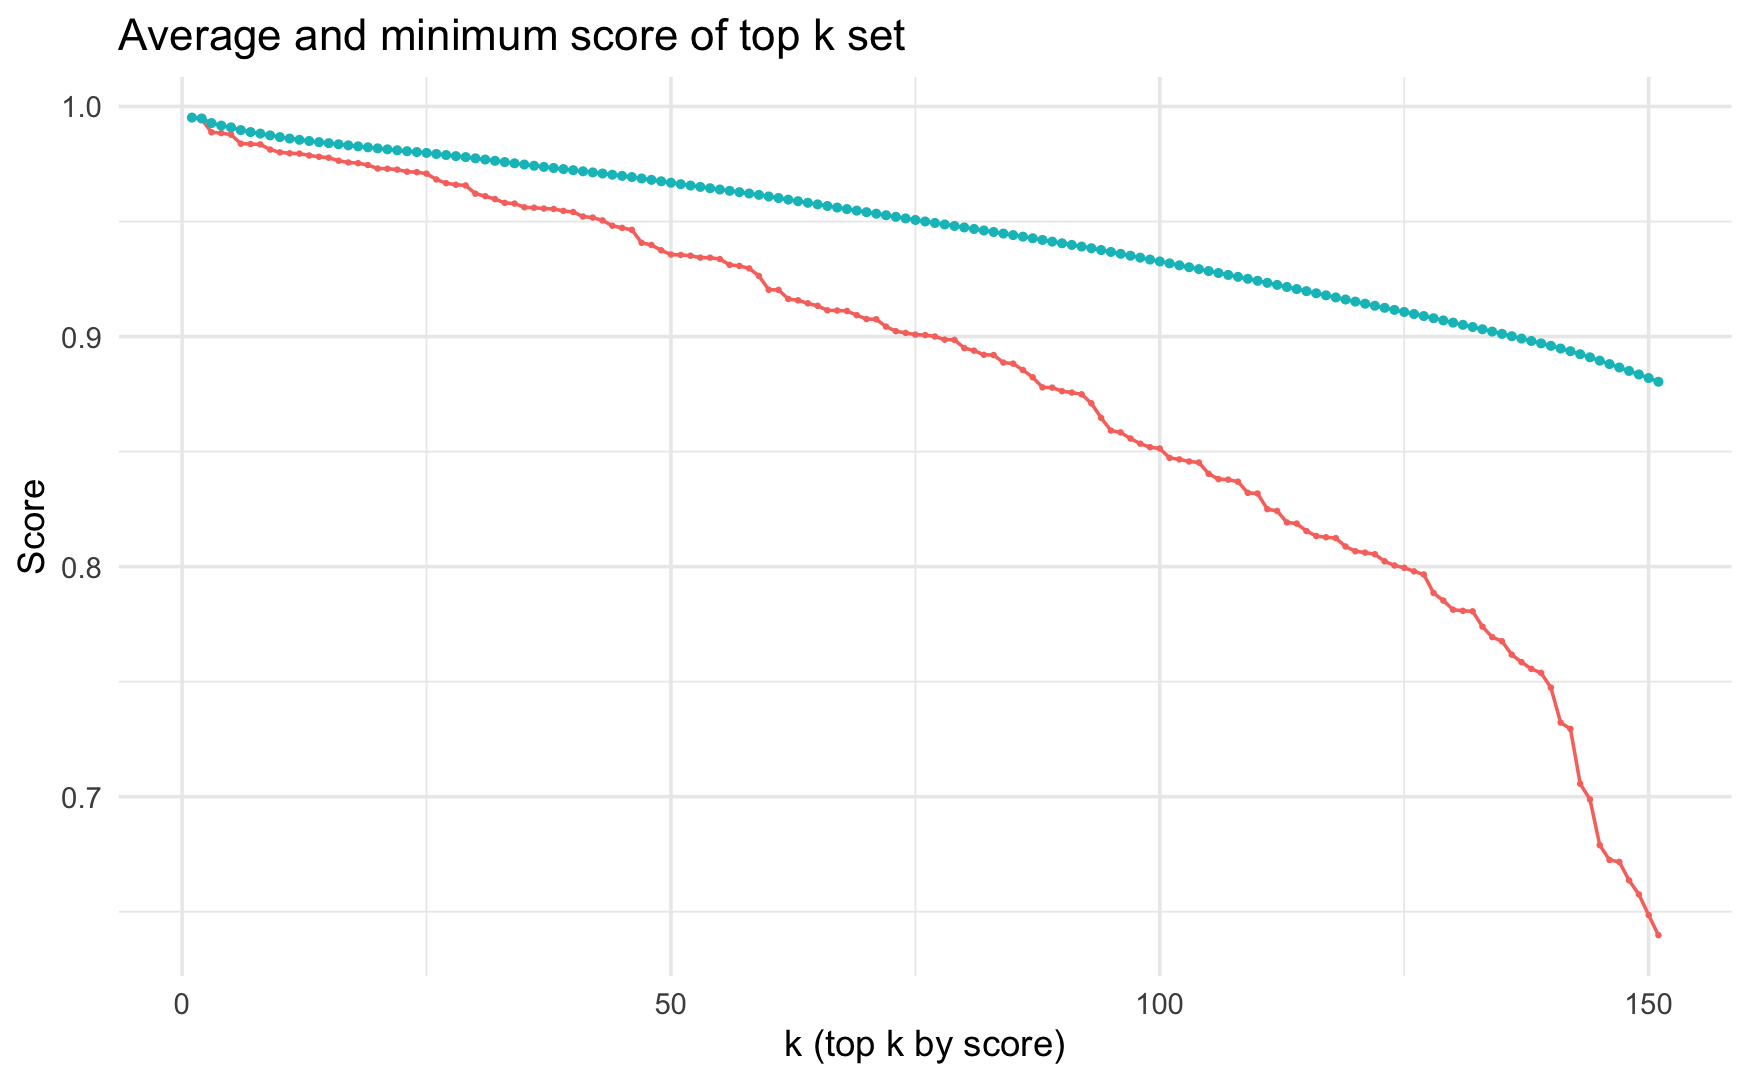
\includegraphics[width=0.8\linewidth]{DominikPlots/sm_score_avg_min.png}
    \caption{Prediction performance (Prediction Set).}
    \label{fig:sm_score_avg_min}
\end{figure}


\subsection{Model Performance}
In the following, we compare the performance of the industry codes selected by the Elastic Net and the Scoring Model. For both approaches, we fit a linear model that includes the selected industry codes together with the lagged main index. Performance is evaluated in terms of mean squared error (MSE), root mean squared error (RMSE), and the coefficient of determination ($R^2$).

\subsubsection{Prediction Set}
For the scoring model we selected the five highest-scoring industry codes at level~2. The selected industries are listed in Table~\ref{tab:sm_sectors}.

\begin{table}[H]
    \centering
    \caption{Industry codes selected by the Scoring Model}
    \label{tab:sm_sectors}
    \small
    \begin{tabularx}{0.9\linewidth}{lX}
        \toprule
        Code & Name \\
        \midrule
        C1620000 & Manufacture of other products of wood; manufacture of articles of cork, straw and plaiting materials \\
        C1720000 & Manufacture of articles of paper and paperboard \\
        C2220000 & Manufacture of plastic products \\
        C2440000 & Manufacture of basic precious and other non-ferrous metals \\
        C2890000 & Manufacture of other special-purpose machinery \\
        \bottomrule
    \end{tabularx}
\end{table}

These industries are predominantly associated with packaging materials, intermediate goods, and investment goods such as machinery. From an economic perspective, this selection is plausible: packaging and input materials are required early in the production process, and machinery is ordered in anticipation of future demand. Consequently, these sectors are likely to lead the overall economic development, with orders placed in advance during expansions and cancelled early in recessions.

The Elastic Net procedure selected a somewhat different set of industries, shown in Table~\ref{tab:en_sectors}. While the codes differ from those identified by the scoring model, the economic interpretation is similar: these industries also represent upstream or investment-oriented activities that tend to react early to changes in the business cycle.

\begin{table}[htbp]
    \centering
    \caption{Industry codes selected by the Elastic Net}
    \label{tab:en_sectors}
    \small
    \begin{tabularx}{0.9\linewidth}{lX}
        \toprule
        Code & Name \\
        \midrule
        C2550000 & Forging, pressing, stamping and roll-forming of metal; powder metallurgy \\
        C2560000 & Treatment and coating of metals; machining \\
        C2840000 & Manufacture of machine tools \\
        C2920000 & Manufacture of bodies (coachwork) for motor vehicles; manufacture of trailers and semitrailers \\
        \bottomrule
    \end{tabularx}
\end{table}

\vspace{\baselineskip}
Because the models differ in the number of predictors, we evaluate performance using $R^2$ rather than adjusted $R^2$. The results are reported in Table~\ref{tab:ps_results}. Both selection methods achieve a higher fit than the benchmark model based solely on the lagged main index. The scoring model performs slightly better than the Elastic Net, although the differences are modest. This outcome is in line with expectations: given its smaller set of selected features, the Elastic Net is likely to perform somewhat worse than the scoring model but still slightly better than the lagged benchmark.

\begin{table}[H]
    \centering
    \caption{Prediction performance (Prediction Set)}
    \label{tab:ps_results}
    \small
    \begin{tabular}{lccc}
        \toprule
         & \textbf{MSE} & \textbf{RMSE} & \textbf{$R^2$}\\
        \midrule
        Scoring Model     & 9.48 & 3.08 & 0.97 \\
        Elastic Net       & 9.99 & 3.16 & 0.96 \\
        Lagged Main Index & 11.00 & 3.32 & 0.96 \\
        \bottomrule
    \end{tabular}
\end{table}

Figure~\ref{fig:ps_pred_performance} plots the model predictions against the observed main index. As expected, all models track the actual development closely. This is not surprising, since a lead of one month is economically short and provides relatively limited scope for divergence.

\begin{figure}[H]
    \centering
    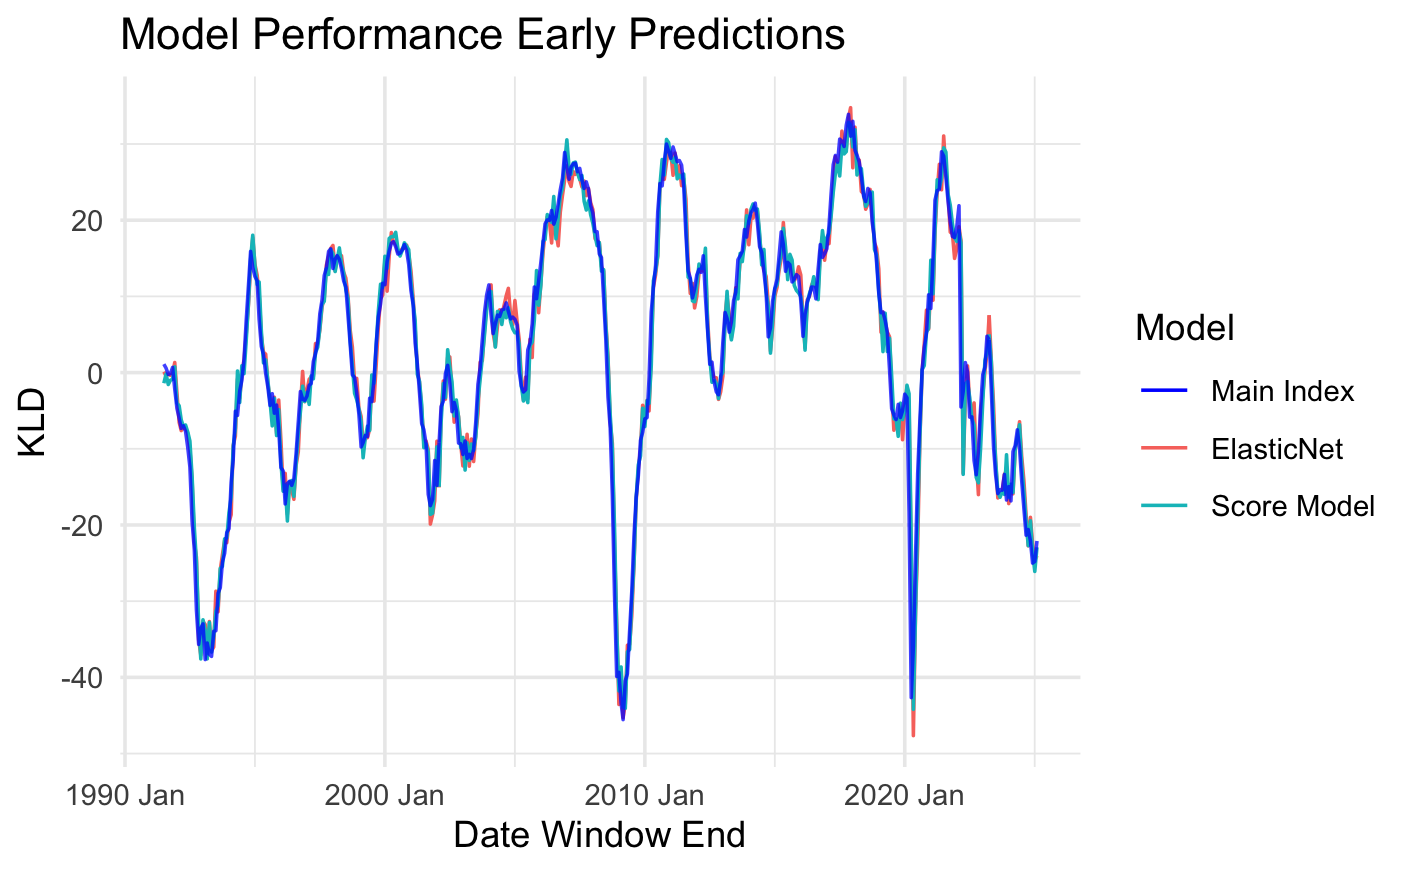
\includegraphics[width=0.8\linewidth]{DominikPlots/ps_pred_performance.png}
    \caption{Prediction performance of different models (Prediction Set).}
    \label{fig:ps_pred_performance}
\end{figure}


\subsubsection{Early Prediction Set}
For the early prediction set we restricted the lead to four to six months, thereby focusing on industries that provide signals further in advance. The selected industries are shown in Tables~\ref{tab:sm_sectors_early} and \ref{tab:en_sectors_early}. While the sets partly differ from those in the general prediction set, there is notable overlap in the types of sectors identified, underlining the same economic reasoning: industries producing upstream inputs or investment goods tend to react early to changes in demand expectations.

\begin{table}[htbp]
    \centering
    \caption{Industry codes selected by the Scoring Model (Early Prediction Set)}
    \label{tab:sm_sectors_early}
    \small
    \begin{tabularx}{0.9\linewidth}{lX}
        \toprule
        Code & Name \\
        \midrule
        C1610000 & Sawmilling and planing of wood \\
        C1710000 & Manufacture of pulp, paper and paperboard \\
        C1720000 & Manufacture of articles of paper and paperboard \\
        C2220000 & Manufacture of plastic products \\
        C2440000 & Manufacture of basic precious and other non-ferrous metals \\
        \bottomrule
    \end{tabularx}
\end{table}

\begin{table}[H]
    \centering
    \caption{Industry codes selected by the Elastic Net (Early Prediction Set)}
    \label{tab:en_sectors_early}
    \small
    \begin{tabularx}{0.9\linewidth}{lX}
        \toprule
        Code & Name \\
        \midrule
        C1610000 & Sawmilling and planing of wood \\
        C2550000 & Forging, pressing, stamping and roll-forming of metal; powder metallurgy \\
        C2560000 & Treatment and coating of metals; machining \\
        C2920000 & Manufacture of bodies (coachwork) for motor vehicles; manufacture of trailers and semitrailers \\
        \bottomrule
    \end{tabularx}
\end{table}

As in the general prediction set, we evaluate the performance of the scoring model, the Elastic Net, and the benchmark model based on lagged values of the main index. The results are summarized in Table~\ref{tab:early_results}. Both selection methods outperform the benchmark, with the scoring model again achieving slightly better predictive accuracy than the Elastic Net.

\begin{table}[H]
    \centering
    \caption{Prediction performance (Early Prediction Set)}
    \label{tab:early_results}
    \small
    \begin{tabular}{lccc}
        \toprule
         & \textbf{MSE} & \textbf{RMSE} & \textbf{$R^2$} \\
        \midrule
        Scoring Model     & 63.00 & 7.94 & 0.77 \\
        Elastic Net       & 66.00 & 8.12 & 0.76 \\
        Lagged Main Index & 79.40 & 8.91 & 0.71 \\
        \bottomrule
    \end{tabular}
\end{table}

Figure~\ref{fig:ps_earlypred_performance} plots the model predictions against the observed main index. Compared to the one-month lead predictions, the increased horizon naturally leads to a lower overall fit. Nonetheless, both the scoring model and the Elastic Net improve substantially over the lagged benchmark, confirming the usefulness of early-predictive industry codes.

\begin{figure}[H]
    \centering
    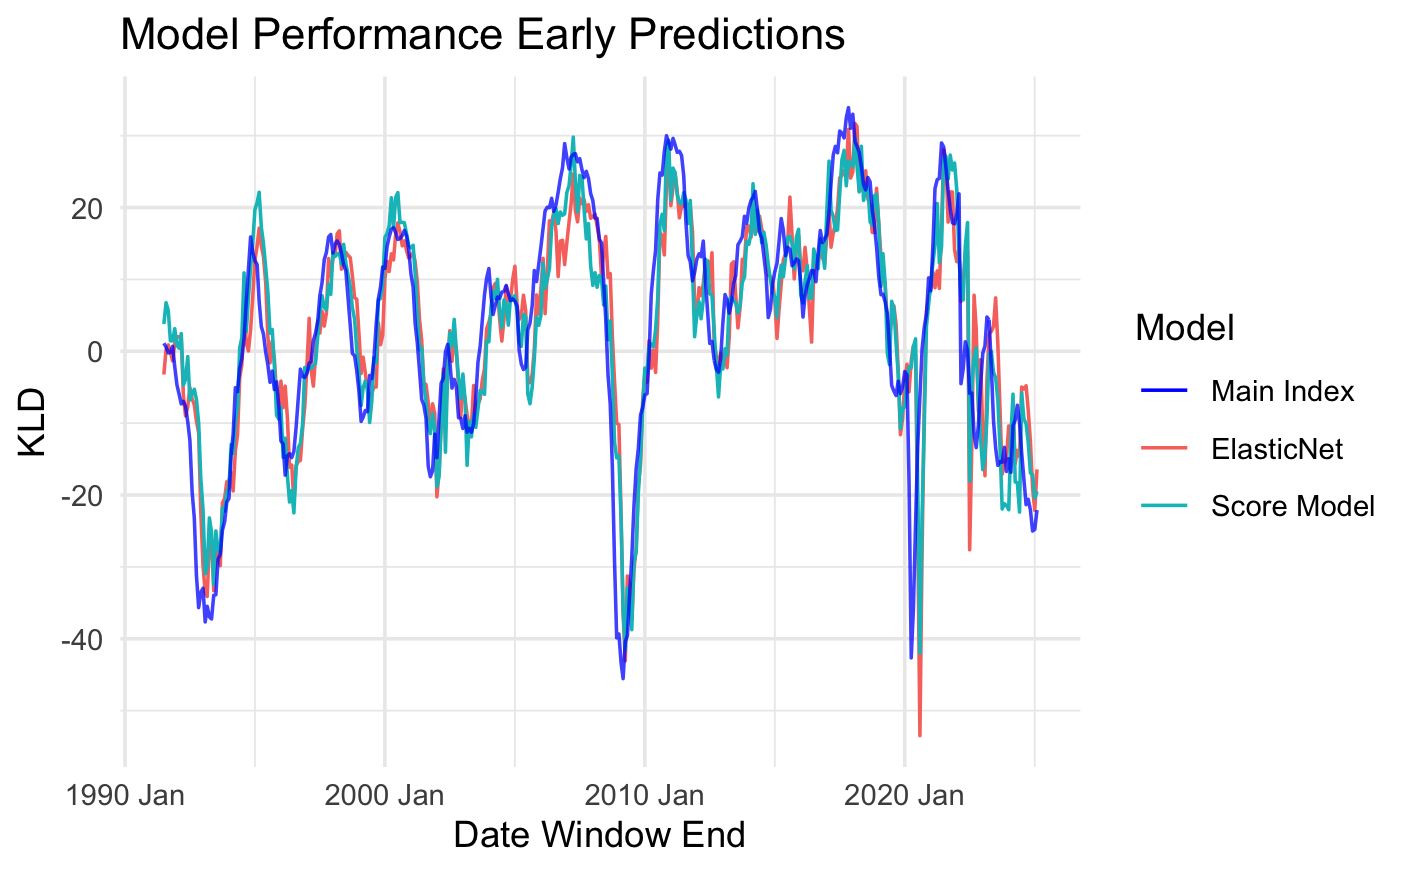
\includegraphics[width=0.8\linewidth]{DominikPlots/ps_earlypred_performance.png}
    \caption{Prediction performance of different models (Early Prediction Set).}
    \label{fig:ps_earlypred_performance}
\end{figure}


\subsubsection{Performance Comparison and Interpretation}

The comparison of cross-correlation profiles highlights important differences between the two selection approaches. As shown in Figures~\ref{fig:comparison_pred_profiles} and \ref{fig:comparison_earlypred_profiles}, the Sparse LM (Elastic Net) identifies industry codes with stronger lead properties, but at the cost of weaker overall correlations. By contrast, the scoring model yields a more robust correlation structure, although peak correlations tend to occur at shorter leads. This reflects the design of the scoring model: by penalizing outliers more heavily, it favors industry codes that exhibit consistently strong correlations across questions and windows, thereby providing a more ``general'' solution.

\begin{figure}[H]
    \centering
    \begin{subfigure}[t]{0.48\linewidth}
        \centering
        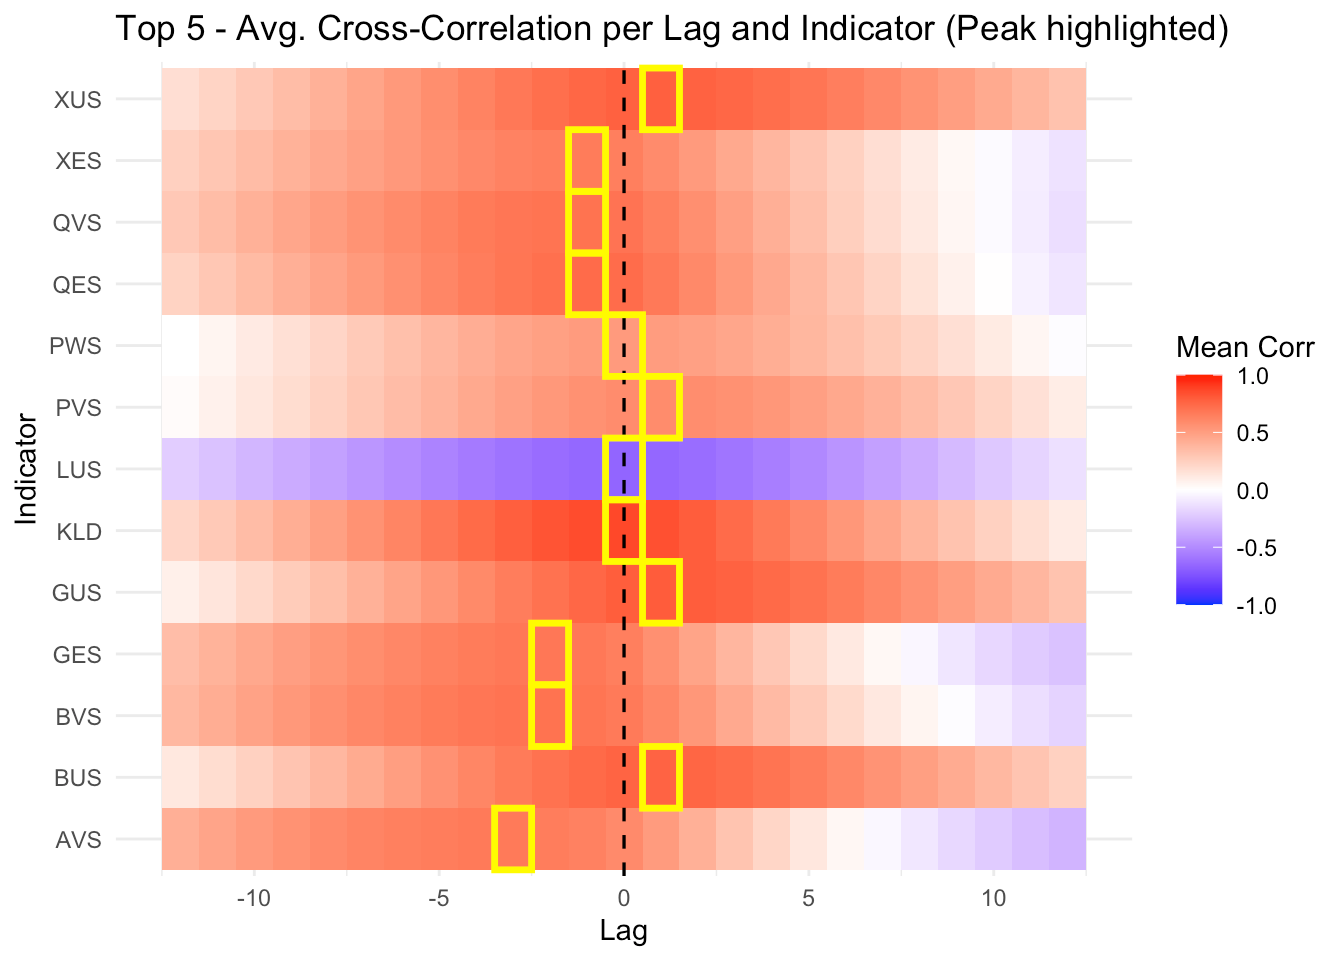
\includegraphics[width=\linewidth]{DominikPlots/ps_score_pred_ccf.png}
        \caption{Prediction Set (Scoring Model).}
        \label{fig:median_score_pred_ps}
    \end{subfigure}%
    \hfill
    \begin{subfigure}[t]{0.48\linewidth}
        \centering
        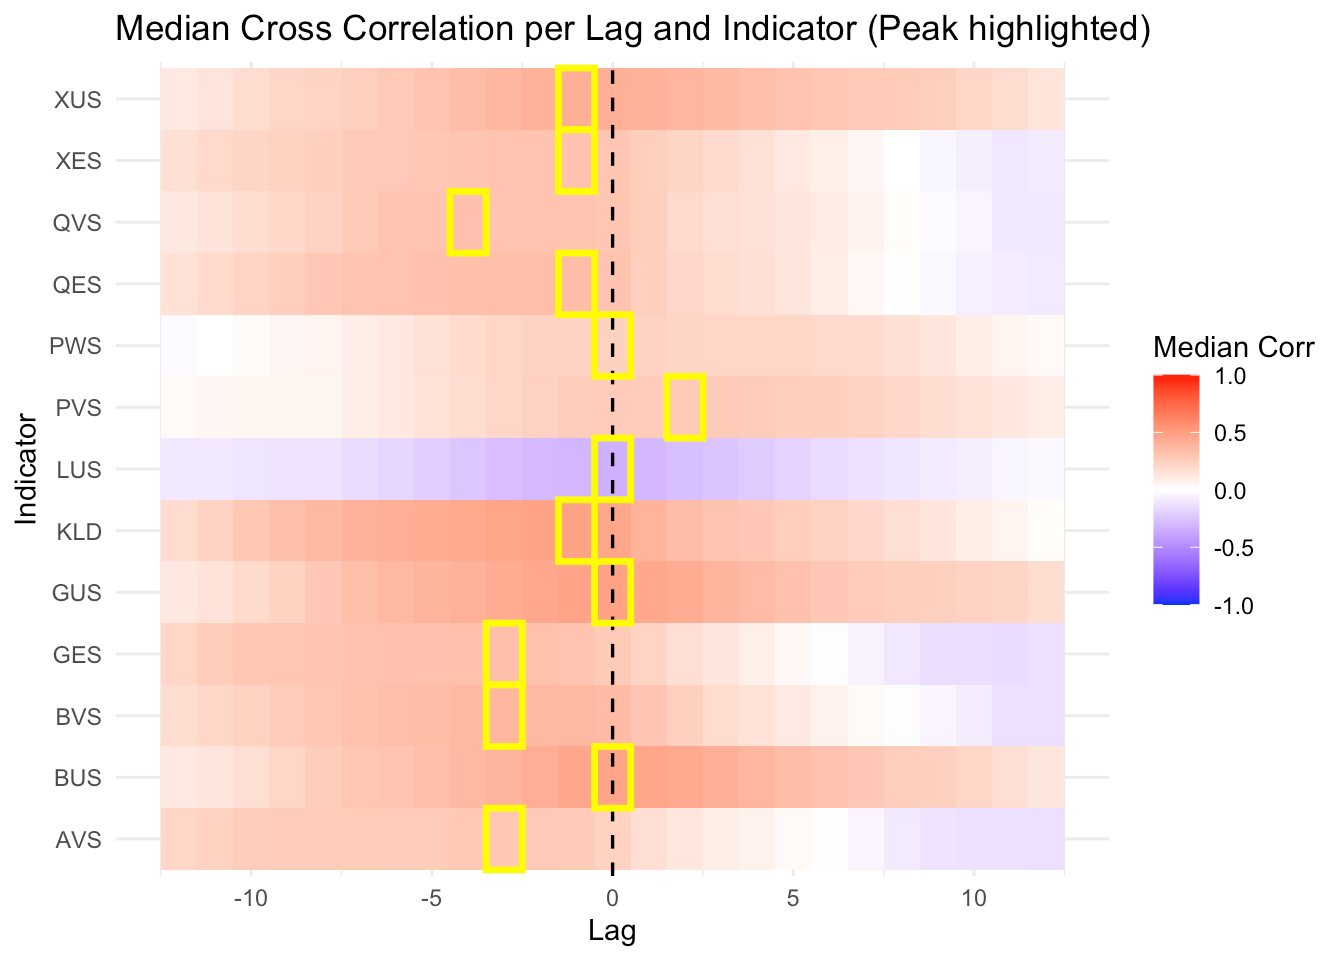
\includegraphics[width=\linewidth]{DominikPlots/ps_lm_pred_ccf.png}
        \caption{Prediction Set (Sparse LM).}
        \label{fig:median_lm_pred_ps}
    \end{subfigure}
    \caption{Comparison of median cross-correlation profiles across industries for the Prediction Set. Yellow boxes indicate peak lags; vertical dashed line marks zero.}
    \label{fig:comparison_pred_profiles}
\end{figure}

\begin{figure}[H]
    \centering
    \begin{subfigure}[t]{0.48\linewidth}
        \centering
        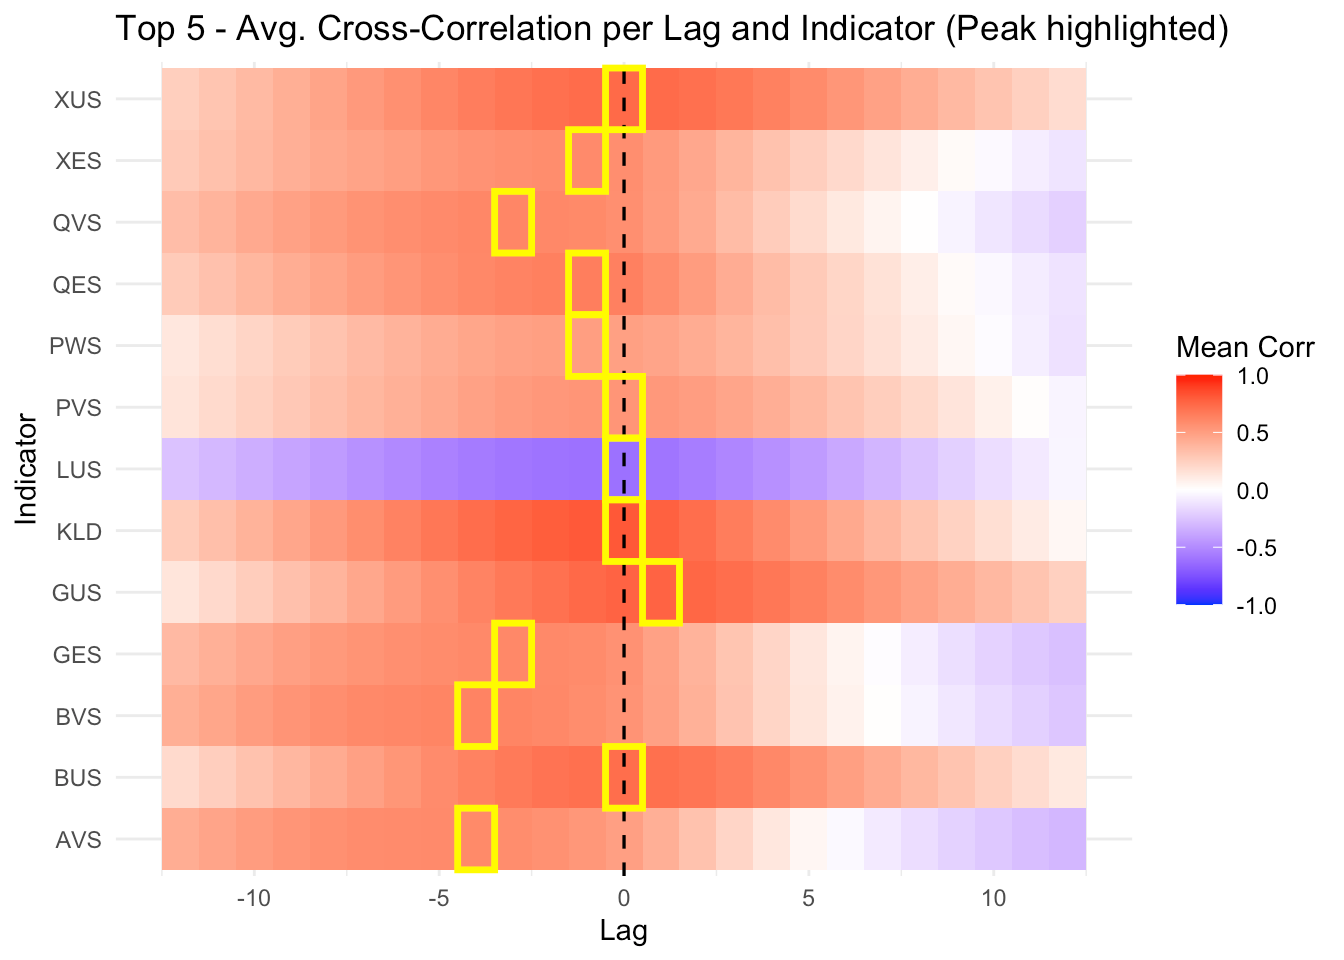
\includegraphics[width=\linewidth]{DominikPlots/ps_score_earlypred_ccf.png}
        \caption{Early Prediction Set (Scoring Model).}
        \label{fig:median_score_pred_early}
    \end{subfigure}%
    \hfill
    \begin{subfigure}[t]{0.48\linewidth}
        \centering
        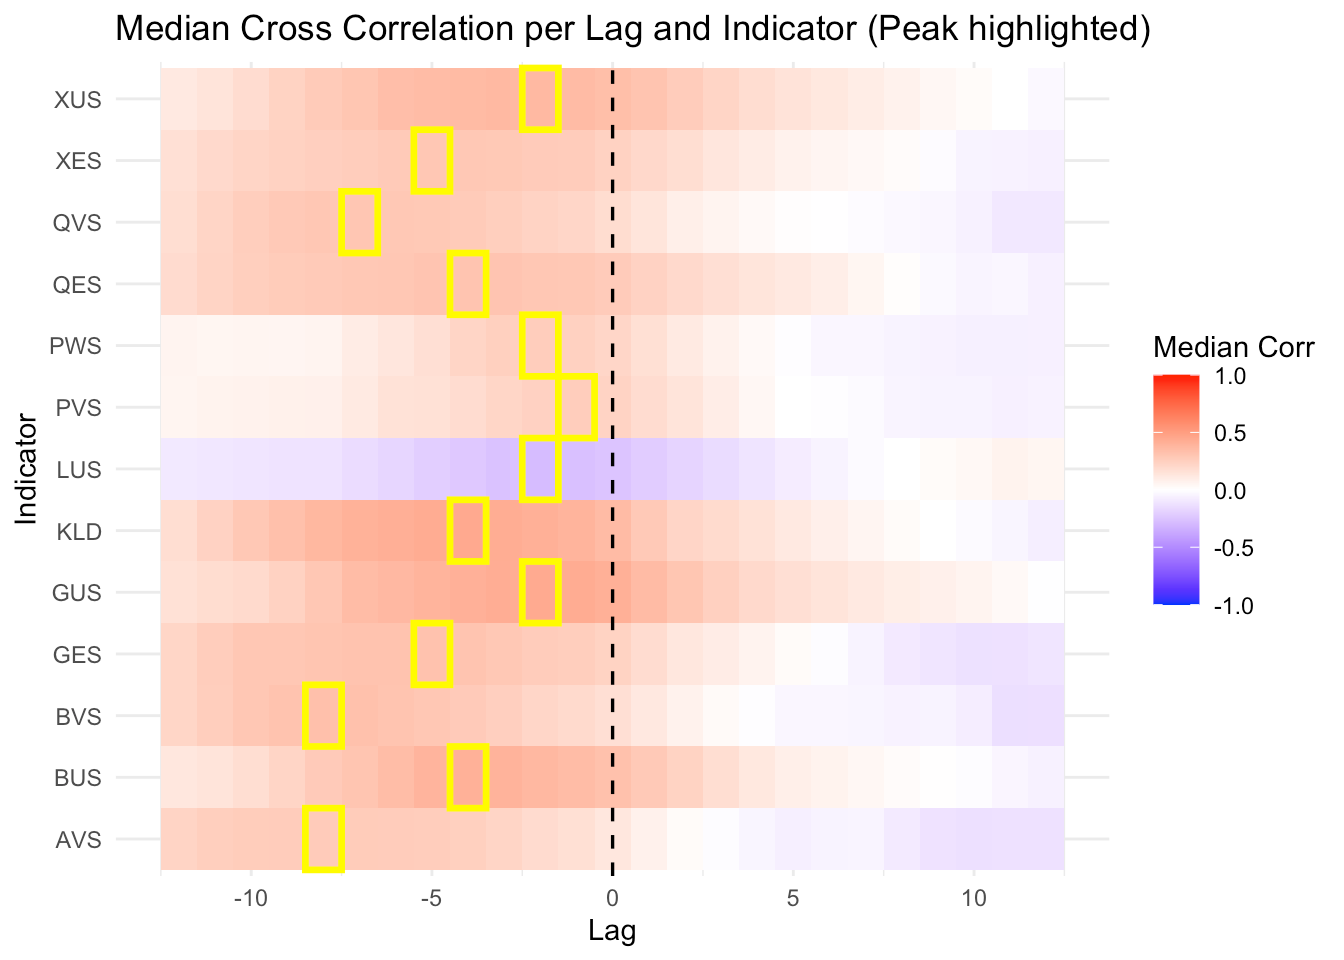
\includegraphics[width=\linewidth]{DominikPlots/ps_lm_earlypred_ccf.png}
        \caption{Early Prediction Set (Sparse LM).}
        \label{fig:median_lm_pred_early}
    \end{subfigure}
    \caption{Comparison of median cross-correlation profiles across industries for the Early Prediction Set (lead 4--6 months).}
    \label{fig:comparison_earlypred_profiles}
\end{figure}

Lagging questions such as BUS and GUS show relatively low lags of peak correlation, illustrating how the two strategies emphasize distinct aspects of predictive performance. The scoring model captures industries with dynamics broadly similar to the main index, which results in highly correlated predictor sets. The $\ell_1$ component underlying the Sparse LM encourages selection of more distinct predictors by retaining one representative from groups of highly correlated industries and discarding the rest; a small $\ell_2$ component (Elastic Net) is included to stabilize estimation under multicollinearity \citep[cf.][]{ZouHastie2005}. This methodological difference helps explain why the selected subsets diverge and why the average correlation strength varies between methods.

To assess robustness, we additionally compare both methods to 500 random subsets of five level-2 industry codes. Figures~\ref{fig:comparison_random_sets}a and~\ref{fig:comparison_random_sets}b display the distribution of $R^2$ across these random subsets. As expected, nearly all subsets outperform the benchmark based solely on lagged main-index values. The scoring model consistently ranks among the stronger subsets, supporting its usefulness as a versatile selection method for predictive modeling.

\begin{figure}[H]
    \centering
    \begin{subfigure}[t]{0.48\linewidth}
        \centering
        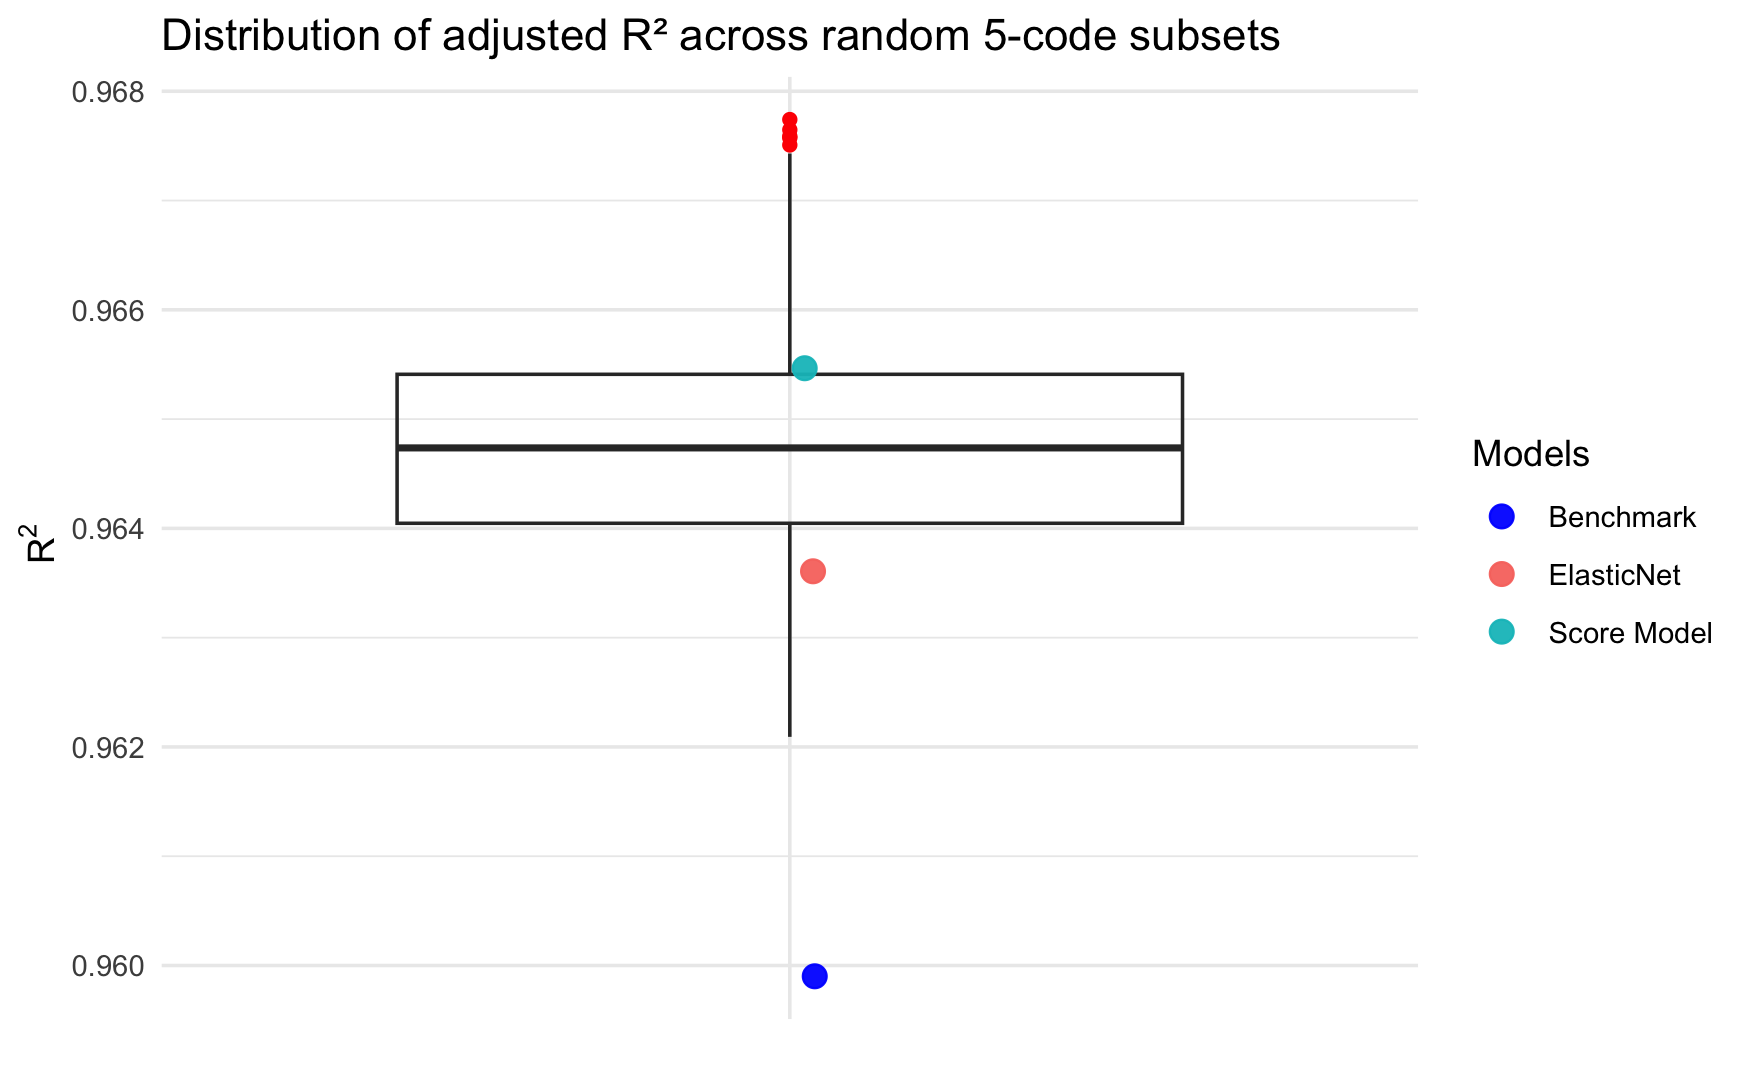
\includegraphics[width=\linewidth]{DominikPlots/ps_pred_random.png}
        \caption{Prediction Set.}
        \label{fig:random_pred}
    \end{subfigure}%
    \hfill
    \begin{subfigure}[t]{0.48\linewidth}
        \centering
        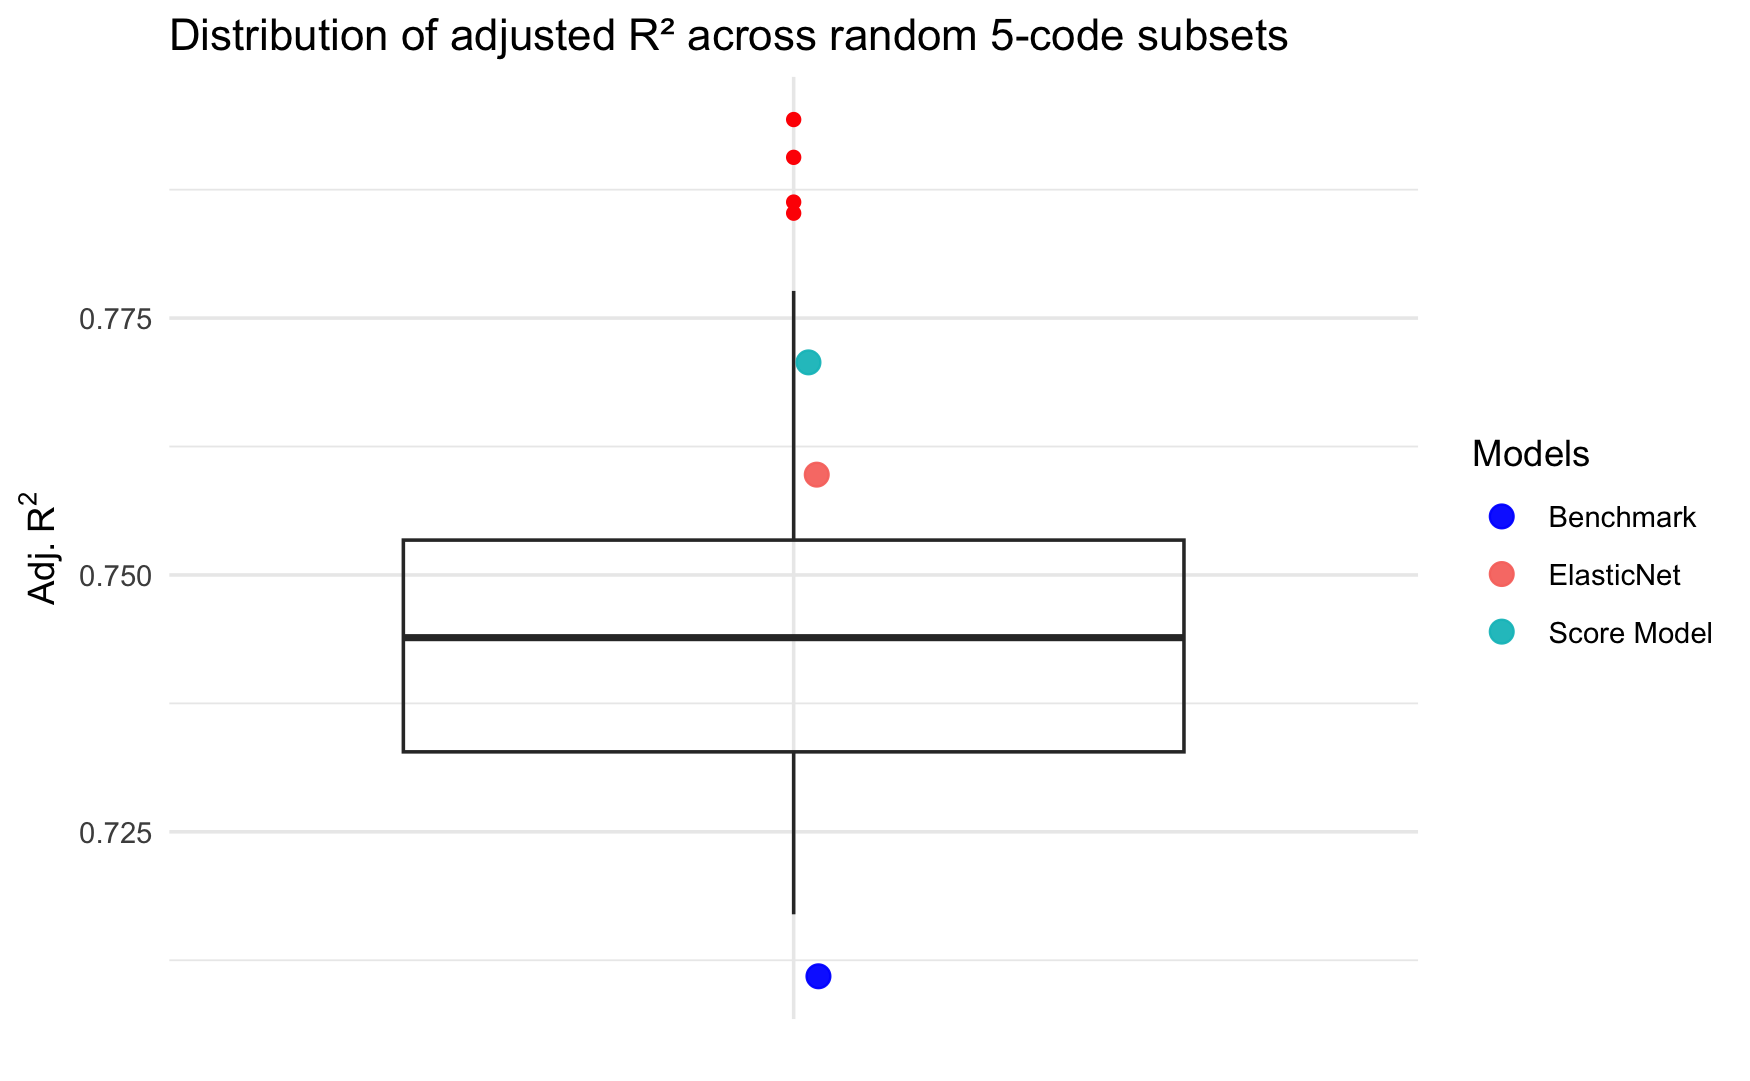
\includegraphics[width=\linewidth]{DominikPlots/ps_earlypred_random.png}
        \caption{Early Prediction Set.}
        \label{fig:random_earlypred}
    \end{subfigure}
    \caption{Distribution of $R^2$ across 500 random 5-code subsets, with benchmark (lagged main index), Elastic Net, and Scoring Model overlaid.}
    \label{fig:comparison_random_sets}
\end{figure}

\vspace{\baselineskip}
At the top end of the distribution, performance is dominated by a small number of outlier subsets. Tables~\ref{tab:random_subsets} and \ref{tab:random_subsets2} list the three best-performing random subsets for the Prediction Set and the Early Prediction Set, respectively. Notably, each table contains twelve distinct industry codes across only three subsets (3$\times$5), indicating that strong predictive performance is not confined to a unique combination of industries. Rather, what matters are shared economic characteristics: upstream inputs, packaging/intermediate goods, and investment-related sectors tend to provide early signals of cyclical turning points.

\begin{table}[H]
    \centering
    \caption{Top 3 random subsets (Prediction Set)}
    \label{tab:random_subsets}
    \small
    \begin{tabularx}{0.9\linewidth}{Xcc}
        \toprule
        \textbf{Industry Codes} & \textbf{$R^2$} & \textbf{RMSE} \\
        \midrule
        C1720000, C2210000, C2590000, C2450000, C2390000 & 0.968 & 2.98 \\
        C1610000, C2740000, C3250000, C2710000, C2450000 & 0.968 & 2.98 \\
        C2570000, C2440000, C1720000, C2310000, C2710000 & 0.968 & 2.98 \\
        \bottomrule
    \end{tabularx}
\end{table}

\begin{table}[H]
    \centering
    \caption{Top 3 random subsets (Early Prediction Set)}
    \label{tab:random_subsets2}
    \small
    \begin{tabularx}{0.9\linewidth}{Xcc}
        \toprule
        \textbf{Industry Codes} & \textbf{$R^2$} & \textbf{RMSE} \\
        \midrule
        C1610000, C2920000, C2910000, C2930000, C1060000 & 0.794 & 7.52 \\
        C2610000, C1610000, C2340000, C1710000, C2310000 & 0.791 & 7.58 \\
        C2550000, C2340000, C3250000, C1610000, C2040000 & 0.786 & 7.66 \\
        \bottomrule
    \end{tabularx}
\end{table}


Multiple paths exist to construct effective predictive sets. The scoring model offers stability and interpretability by selecting industries with consistently strong correlations to the main index across questions and windows. The Elastic Net (Sparse LM) promotes diversity by emphasizing distinct predictors and stabilizes estimation via an additional $\ell_2$ component. Random subsets demonstrate that predictive skill is widely distributed across industries, yet especially pronounced among upstream and investment-oriented sectors.

\newpage
\subsection{Clustering based on CCF}
So far, we have mostly considered all questions within each industry. To find potentially leading groups, which can contain different questions of different industries, we took on a clustering approach based their relationship with the main index. We computed the CCF of all individual questions of all level 2 aggregates and then performed Ward's method to cluster them \citep{ward1963hierarchical}. In a nutshell, Ward's method starts with each component as its own cluster and iteratively merges clusters in a way that minimizes the overall within-cluster variance.

\subsubsection{Comparing cluster groups}
A challenge lied in finding a good measure to compare the resulting groups and rank out potentially interesting ones. Simply ranking clusters by correlation strength does not distinguish between leading and lagging behavior. To address this, we adopted a similar strategy as in the previous methods: we fitted a linear model predicting the main index $y$ using its own lagged values along with the lagged values of a cluster average $x$ up to lag $k$:
\[
y_t \sim y_{t-1} + y_{t-2} + ... + y_{t-k} + x_{t-1} + x_{t-2} + ... + x_{t-k} 
\]
Again, we used one setting with all lagged values up to 6 months behind and another early setting, where we only considered lags 4 to 6. Table~\ref{tab:clusterMSE} shows the top 5 clusters according to the MSE of the above model for both settings. 
\begin{table}[H]
\centering
\small
\begin{subtable}{0.48\textwidth}
\centering
\begin{tabular}{c c c c c}
\toprule
Cluster & $n$ & MSE & RMSE& Adj. $R^{2}$ \\
\midrule
2  & 9 & 10.27 & 3.21 & 0.9615 \\
10 & 9 & 10.31 & 3.21 & 0.9613 \\
16 & 7 & 10.32 & 3.21 & 0.9613 \\
63 & 8 & 10.37 & 3.22 & 0.9611 \\
62 & 5 & 10.41 & 3.23 & 0.9609 \\
\midrule
Lagged Main & 1 & 11.00 & 3.32 & 0.959 \\
\bottomrule
\end{tabular}
\caption{Considering lags 1 to 6.}
\end{subtable}\hfill
\begin{subtable}{0.48\textwidth}
\centering
\begin{tabular}{c c c c c}
\toprule
Cluster & $n$ & MSE & RMSE & Adj. $R^{2}$ \\
\midrule
63 & 8  & 65.39 & 8.09 & 0.758 \\
48 & 4  & 66.18 & 8.14 & 0.755 \\
1  & 8  & 67.46 & 8.21 & 0.751 \\
3  & 12 & 67.72 & 8.23 & 0.750 \\
5  & 10 & 69.97 & 8.36 & 0.741 \\
\midrule
Lagged Main  & 1 & 79.4 & 8.91 & 0.70\\
\bottomrule
\end{tabular}
\caption{Considering lags 4 to 6}
\end{subtable}
\caption{Top 5 clusters based on MSE}
\label{tab:clusterMSE}
\end{table}

The predictive performance of the above model alone is not necessarily a sufficient indicator to find a meaningfully leading group. Lagged values of a cluster average could add relevant information to the lagged values of the main index, resulting in a low MSE, while still not leading the main index. A visual examination of the CCFs of the cluster can help in further determining leading clusters. Fig.~\ref{fig:cluster_ccf} shows the CCFs of the clusters from table~\ref{tab:clusterMSE}. As expected, more of the top 5 clusters of the early prediction setting seem to be  leading, compared to the other setting. 

\begin{figure}[H]
\centering
\begin{subfigure}{0.48\textwidth}
  \centering
  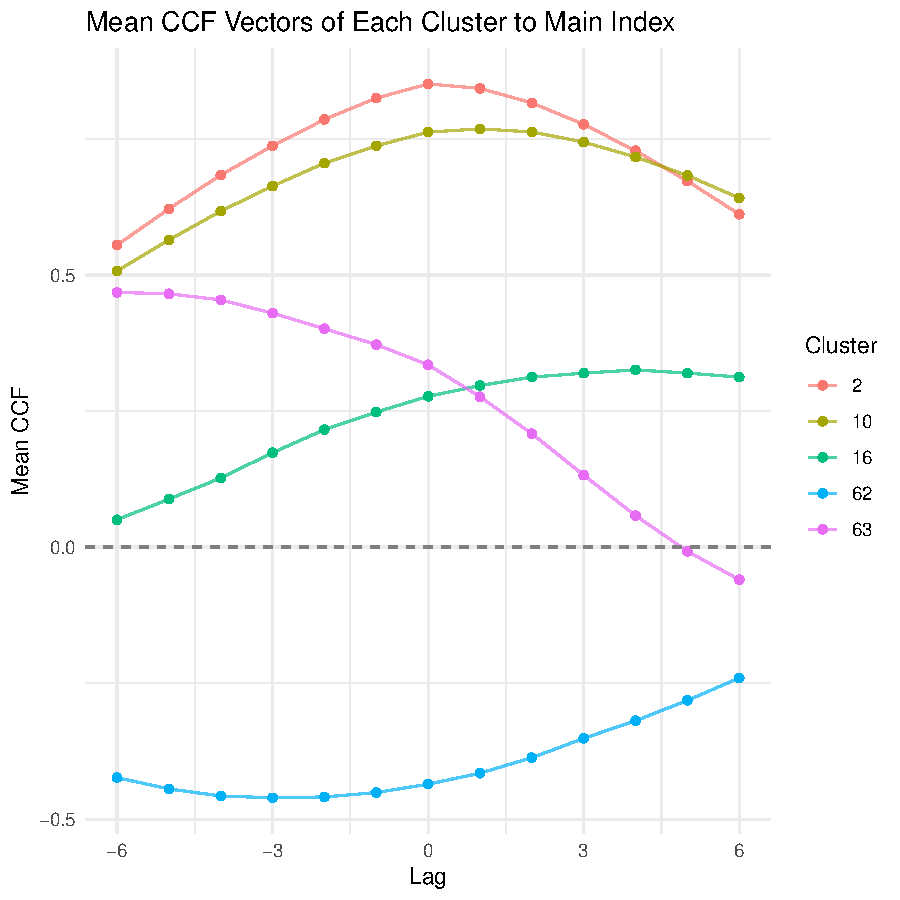
\includegraphics[width=\linewidth]{JakobPlots/ccfs_cluster_plot_1_6.pdf}
  \caption{Top 5 clusters.}
\end{subfigure}\hfill
\begin{subfigure}{0.48\textwidth}
  \centering
  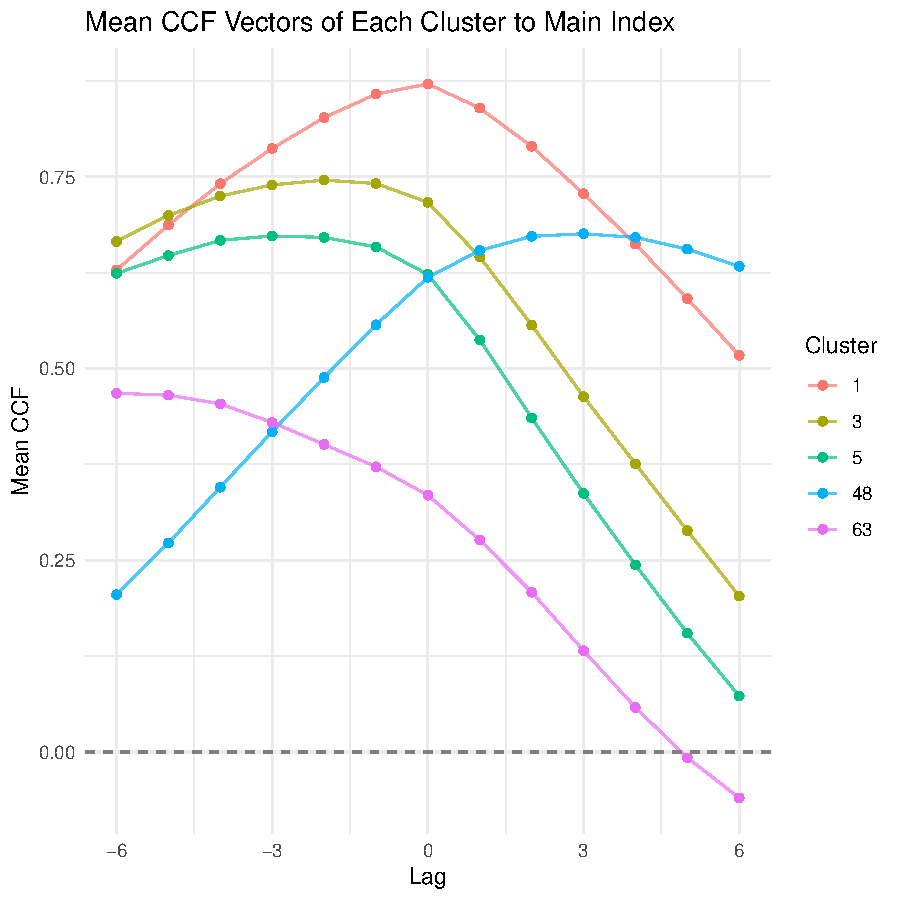
\includegraphics[width=\linewidth]{JakobPlots/ccfs_cluster_plot_4_6.pdf}
  \caption{Top 5 early-predictor clusters.}
\end{subfigure}
\caption{Mean CCFs of the top 5 cluster averages.}
\label{fig:cluster_ccf}
\end{figure}

\subsubsection{Exemplary Cluster}
Although most clusters are difficult to interpret, cluster 3 from the top 5 provides an illustrative example of a potentially meaningful grouping. As shown in Fig.~\ref{fig:cluster3}, the series in this cluster tend to lead the main index, while Table~\ref{tab:cluster3_components} details its constituent components. Its dominated by questions which compare the current situation to the previous month and many of the industries deal with intermediate components or capital goods.

\begin{figure}[H]
    \centering
    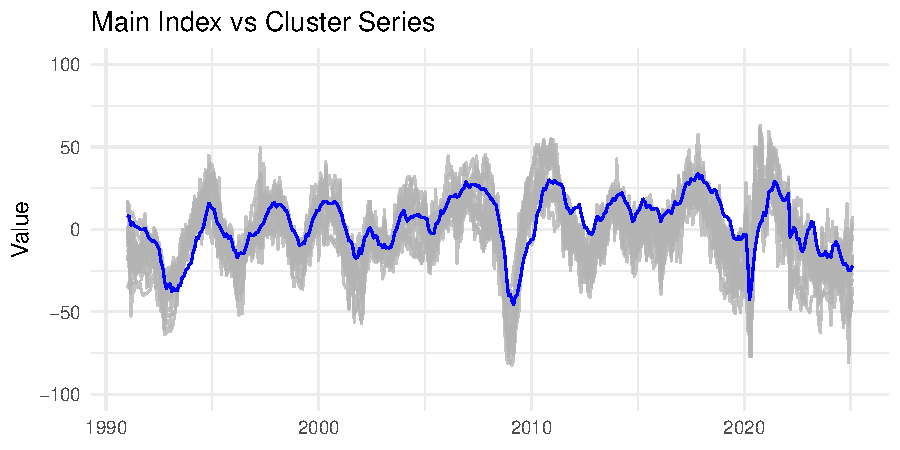
\includegraphics[width=0.8\linewidth]{JakobPlots/3main_plot.pdf}
    \caption{Main index (blue) vs individual series in cluster 3.}
    \label{fig:cluster3}
\end{figure}

\begin{table}[H]
\centering
\footnotesize
\begin{tabular}{ll}
\toprule
\textbf{Industry Title} & \textbf{Question Title} \\
\midrule
Manufacture of plastic products & Business situation expectations \\
Manufacture of plastic products & Order backlog compared to previous month \\
Manufacture of plastic products & Production compared to previous month \\
Manufacture of forged, pressed, drawn, and stamped parts & Order backlog compared to previous month \\
Manufacture of forged, pressed, drawn, and stamped parts & Production compared to previous month \\
Manufacture of forged, pressed, drawn, and stamped parts & Production plans \\
Manufacture of cutlery, tools, and locks & Business situation expectations \\
Manufacture of cutlery, tools, and locks & Demand compared to previous month \\
Manufacture of electric motors, generators, transformers, etc. & Demand compared to previous month \\
Manufacture of non-industry-specific machinery & Demand compared to previous month \\
Manufacture of machine tools & Business situation expectations \\
Paper, cardboard, and paperboard processing & Order backlog compared to previous month \\
\bottomrule
\end{tabular}
\caption{Individual series present in cluster 3.}
\label{tab:cluster3_components}
\end{table}